% Autogenerated translation of 语法分析.md by Texpad
% To stop this file being overwritten during the typeset process, please move or remove this header

\documentclass[12pt]{book}
\usepackage{graphicx}
\usepackage{fontspec}
\usepackage[utf8]{inputenc}
\usepackage[a4paper,left=.5in,right=.5in,top=.3in,bottom=0.3in]{geometry}
\setlength\parindent{0pt}
\setlength{\parskip}{\baselineskip}
\setmainfont{Helvetica Neue}
\usepackage{hyperref}
\pagestyle{plain}
\begin{document}

\chapter*{概述}

\section*{功能}

以词法分析得到的记号序列为输入,构建分析树。与此同时还要进行语法检查、错误处理。

\section*{分析顺序}

分析时对输入符号串的扫描是自左向右进行的,记为L。对于自顶向下的分析方法,构造出的是一个最左推导序列,因此记为LL。而对于自底向上的分析方法,构造出的是一个最右推导的逆过程,因此记为LR。

\subsection*{自顶向下的分析方法}

以由顶向下的顺序构造分析树。如:对于文法

\$S→aAcBe\$
\$A→b$\vert$Ab\$
\$B→d\$

一个自顶向下的分析序列为:

\$S→aAcBe→aAbcBe→abbcBe→abbcde\$

是一个最左推导。

\subsection*{自底向上的分析方法}

以自底向上的顺序构造分析树,如一个自底向上的分析序列为:

\$abbcde→aAbcde→aAcde→aAcBe→S\$

是一个最右推导的逆过程。

\section*{错误处理}

\begin{itemize}
\item 紧急恢复:发现错误后不断丢弃输入符号,直到向前指针指向某个定界符,如分号、块结束标识END等。
\item 短语级恢复:对剩余输入符号串的前缀进行局部修改,使得其可以满足语法分析程序的继续。如将逗号改为分号,去除多余的逗号等。
\item 出错产生式:扩充语法,直接对错误进行识别,然后进行相应处理。
\item 全局纠正:尝试找出能使分析程序继续下去的最少的对剩余输入串的修改。难以实现。
\end{itemize}

\chapter*{自顶向下分析}

模拟生成树从上到下的构造过程,有不看输入符号串,枚举不同推导方式的递归下降分析,以及通过向前看若干个符号,每一步都得到唯一确定的推导方式的预测分析。

\section*{递归下降分析}

本质上就是枚举文法的所有情况找到符合输入符号串的分析树。过程中需要不断试探、回溯,效率太低,极少采用。

\section*{消除回溯}

为了得到效率更高的分析方法,首先要消除回溯。要消除回溯,首先要修改文法,使得分析过程的每一步都是确定的。这要求文法:
- 不含二义性
- 不含左递归
- 每个非终结符号的所有推导,开头的终结符两两互不相交。即:对于每一个产生式\$A rightarrow alpha\emph{1left$\vert$alpha}2right$\vert$ ldots mid alpha\emph{n\$,有\$operatorname\{FIRST\}left(alpha}\{boldsymbol\{i\}\}right) cap operatorname\{FIRST\}left(alpha\_\{boldsymbol\{j\}\}right)=phi quad(mathbf\{i\} neq mathbf\{j\})\$

\subsection*{概念}

\begin{itemize}
\item FIRST集
\end{itemize}

  \$FIRSTleft(alpha\emph{iright)=left\{a mid alpha}i stackrel\{\emph{\}\{rightarrow\} a beta, a in V\emph{T, alpha}i 、 beta inleft(V\emph{T cup V}Nright)\textasciicircum{}}right\}\$

  如果\$alpha\emph{i stackrel\{*\}\{Rightarrow\} varepsilon\$,则规定\$varepsilon in FIRST left(alpha}iright)\$

\begin{itemize}
\item FOLLOW集
\end{itemize}

  \$FOLLOW(A)=left\{a mid S stackrel\{*\}\{Rightarrow\} ldots text \{ Aa \} ldots, a in V\_Tright\}\$

\subsection*{算法}

\begin{itemize}
\item 消除左递归:假定关于 \$A\$ 的全部产生式是:
\$\$
A rightarrow A alpha\emph{1left$\vert$ A alpha}2right$\vert$ ldotsleft$\vert$ A alpha\emph{\{ m \}right$\vert$ beta}1left$\vert$beta\emph{2right$\vert$ ldots mid beta}n
\$\$
产生式可以改写为:
\$\$
begin\{aligned\}
\& A rightarrow beta\emph{1 A \textasciicircum{}\{prime\}left$\vert$beta}2 A \textasciicircum{}\{prime\}right$\vert$ ldots mid beta\emph{n A \textasciicircum{}\{prime\} \textbackslash{}
\& A \textasciicircum{}\{prime\} rightarrow alpha}1 A \textasciicircum{}\{prime\}left$\vert$alpha\emph{2 A \textasciicircum{}\{prime\}right$\vert$ ldotsleft$\vert$alpha}m A \textasciicircum{}\{prime\}right$\vert$ varepsilon
end\{aligned\}
\$\$
\item 提取左公因子:若有产生式
\$\$
A rightarrow alpha beta\emph{1left$\vert$alpha beta}2right$\vert$ ldotsleft$\vert$alpha beta\emph{nright$\vert$ gamma
\$\$
可改写为:
\$\$
begin\{aligned\}
\& A rightarrow alpha A \textasciicircum{}\{prime\} mid gamma \textbackslash{}
\& A \textasciicircum{}\{prime\} rightarrow beta}1left$\vert$beta\emph{2right$\vert$ ldots mid beta}n
end\{aligned\}
\$\$
\end{itemize}

\section*{递归调用预测分析}

消除回溯后,一个简单的想法是为每一个非终结符\$A\$构造其状态转换图,编写其对应的函数,用于识别其句子。该函数每次向前看一个输入符号\$a\$,选择状态转换图中与之相符的边,

\begin{itemize}
\item 若边为终结符,则指针后移,读入下一个输入符号。
\item 若边为非终结符,则调用该非终结符的对应函数。
\item 若不存在符合的边,则若生成式中包含\$Arightarrowvarepsilon\$,则结束函数。否则报错。
\end{itemize}

上述方法要能够实现,要求每个非终结符的状态转移图中,每个状态节点的射出边都不同名,不存在标记为\$varepsilon\$的边,且若存在非终结符边,则该边是唯一射出边。

\section*{非递归预测分析}

上述方法中,函数间的递归调用会浪费资源,且限制了当状态节点的射出边为非终结符时不能有其他射出边。另一种方法是:利用栈保存文法分析的状态,利用预测分析表决定行为,也就是下面的LL(1)分析方法。

\chapter*{LL(1)分析}

LL(1)分析属于非递归预测分析,利用栈和预测分析表完成分析树的构造。L、L、(1)分别表示扫描顺序自左向右、分析顺序为最左推导、每次做决定时向前看一个符号。

\section*{预测分析表}

行为栈顶非终结符的符号,列为待输入串的首个符号(包括\$\$\$),内容为需要用到的生成式,如:

\includegraphics{media/%E8%AF%AD%E6%B3%95%E5%88%86%E6%9E%90/Image%20From%20Chapter+04--%E8%AF%AD%E6%B3%95%E5%88%86%E6%9E%90.png}

\section*{预测分析表的构造}

\subsection*{FIRST集合及其构造}

\begin{itemize}
\item FIRST集的定义:开头终结符号的集合\textbf{(包括\$varepsilon\$)}
\$operatorname\{FIRST\}left(alpha\emph{iright)=left\{a mid alpha}i stackrel\{\emph{\}\{rightarrow\} a beta, a in V\emph{\{mathrm\{T\}\}, alpha}i 、 beta inleft(V\emph{\{mathrm\{T\}\} cup V}\{mathrm\{N\}\}right)\textasciicircum{}}right\}\$
如果\$alpha\emph{i stackrel\{*\}\{Rightarrow\} varepsilon\$,则规定\$varepsilon in FIRST left(alpha}iright)\$
\item FIRST集的构造

\begin{itemize}
\item 若\$X in V\_T\$,则\$FIRST(X)=\{X\}\$
\item 若 \$X in V\emph{N\$, 且有产生式 \$X rightarrow a . .\$,其中 \$a in V}T\$, 则把 \$a\$ 加入到\$FIRST(X)\$中
\item 若 \$X rightarrow varepsilon\$ 也是产生式, 则 \$varepsilon\$ 也加入到\$FIRST(X)\$中
\item 若 \$X rightarrow Y ldots\$ 是产生式, 且 \$Y in V\_N\$ ,则把\$FIRST(Y)\$ 中的所有非\$varepsilon\$元素加入到\$FIRST(X)\$中
\item 若 \$X rightarrow Y\emph{1 Y}2 ldots Y\emph{k\$ 是产生式, 如果对某个 \$i\$,
\$FIRSTleft(Y}1right)、 FIRSTleft(Y\emph{2right)、ldots、FIRSTleft(Y}\{i-1\}right)\$ 都含有 \$varepsilon\$, 即 \$Y\emph{1 Y}2 ldots Y\emph{\{i-1\} stackrel\{*\}\{Rightarrow\} varepsilon\$,
则把\$FIRSTleft(Y}iright)\$ 中的所有非 \$varepsilon\$ 元素加入到\$FIRST(X) \$中
\item 若所有 \$FIRSTleft(Y\_iright)\$ 均含有 \$varepsilon\$, 其中 \$i=1、2、ldots k\$, 则把 \$varepsilon\$ 加入到\$FIRST(X)\$中
\end{itemize}
\end{itemize}

\subsection*{FOLLOW集合及其构造}

\begin{itemize}
\item FOLLOW集的定义:尾随的终结符号集合\textbf{(包括\$\$\$,不包括\$varepsilon\$)}
\$FOLLOW(A)=left\{a mid S stackrel\{\emph{\}\{Rightarrow\} ldots text \{ Aa \} ldots, a in V\_Tright\}\$
若\$mathrm\{S\} stackrel\{}\}\{Rightarrow\} ldots mathrm\{A\}\$,则规定\$\$ in FOLLOW (A)\$,\$\$\$是输入串结束的标识符
\item FOLLOW集的构造

\begin{itemize}
\item 对文法开始符号S,置\$\$\$于\$FOLLOW(S)\$中, \$\$\$为输入符号串的右尾标志
\item 若 \$A rightarrow alpha B beta\$ 是产生式, 则把\$FIRST(beta)\$ 中的所有非 \$varepsilon\$ 元素加入到\$FOLLOW(B)\$中
\item 若 \$A rightarrow alpha B\$ 是产生式, 或 \$A rightarrow alpha B beta\$ 是产生式并且 \$beta stackrel\{*\}\{Rightarrow\} varepsilon\$, 则把\$FOLLOW(A)\$中的所有元素加入到\$FOLLOW(B)\$中
\item 重复此过程, 直到所有集合不再变化为止
\end{itemize}
\end{itemize}

\subsection*{预测分析表的构造}

for (文法G的每个产生式A→\$alpha\$)
\{
	for (每个终结符号\$a in FIRST(alpha)\$)
		把\$A→alpha\$放入\$M[A, a]\$中;
	if (\$varepsilon in FIRST(alpha)\$)
		for (任何 \$bin FOLLOW(A)\$)
			把 \$A→alpha\$放入\$M[A, b]\$中;
\}
for (所有无定义的\$M[A, a]\$)
	标上错误标志;

\section*{预测分析控制程序}

首先将\$\$\$入栈,再将起始符号\$S\$入栈。

然后根据循环下列过程:记栈顶符号为X,待输入串第一个符号为a

\begin{itemize}
\item 若X为终结符且X==a,则该符号退栈,输入指针前移
\item 若X为终结符且X!=a,出错
\item 若X=a=\$\$\$,则分析成功
\item 若X为非终结符,则访问分析表M[X,a]

\begin{itemize}
\item M[X,a]为\$varepsilon\$,则将X退栈
\item M[X,a]不为\$varepsilon\$,\$M[X, a]=X→Y\emph{1Y}2...Y\emph{n\$,则将生成式右部符号反向入栈,即\$Y}1\$最终会在栈顶
\item M[X,a]不存在,出错
\end{itemize}
\end{itemize}

\section*{错误处理}

\begin{itemize}
\item X为终结符且X!=a:将X弹出
\item X为非终结符但M[X,a]不存在:若a在X的FOLLOW集中,则弹出X,否则跳过a。可以通过在分析表中加入同步化信息实现:对于\$Ain V\_N\$,\$bin FOLLOW(A)\$,若M[A, b]为空,则加入“synch”。
\end{itemize}

\section*{LL(1)文法}

利用上述方法构造预测分析表后,表中不为空的每一项都是唯一的,则该文法为LL(1)文法。也可以用以下规则判断:

一个文法是LL(1)文法,当且仅当它的每一个产生式\$A→alphamidbeta\$,满足:

\begin{itemize}
\item \$FIRST(alpha) cap FIRST(beta)=phi\$,并且
\item 若 \$beta\$ 推导出 \$varepsilon\$, 则\$FIRST(alpha) cap FOLLOW(A)=phi\$
\end{itemize}

\chapter*{自底向上分析法}

基本思想是由输入串出发,每次规约一个最左直接短语,最终得到起始符号,从而得到分析树,本质上是最右推导的逆过程。

\section*{概念}

\subsection*{句型,句子和语言}

\begin{itemize}
\item 一个文法推导过程中可能出现的符号序列为句型。最左推导得到的是左句型,最右推导得到的是右句型
\item 仅含有终结符号的句型是文法的一个句子
\item 文法所能产生的所有句子的集合称为语言
\end{itemize}

\subsection*{短语,直接短语和句柄}

\begin{itemize}
\item 文法推导过程中某个非终结符号经过若干次推导得到的符号序列称为短语。推导次数为1的称为直接短语。即:对于文法 \$G =left( V \_\{ T \}, V \_\{ N \}, S , varphiright)\$,假定 \$alpha beta delta\$ 是文法 \$G\$ 的一个句型, 如果存在:
\$\$
S stackrel\{\emph{\}\{Rightarrow\} alpha A delta text \{, 并且 \} A stackrel\{+\}\{Rightarrow\} beta
\$\$
则称 \$beta\$ 是句型 \$alpha beta delta\$ 关于非终结符号 \$A\$ 的短语。
如果存在:
\$\$
S stackrel\{}\}\{Rightarrow\} alpha A delta, text \{ 并且 \} A Rightarrow beta
\$\$
则称 \$beta\$ 是句型 \$alpha beta delta\$ 关于非终结符号 \$A\$ 的直接短语。
\item 一个句型的最左直接短语称为该句型的句柄。也就是最左推导中每一步由非终结符得到的生成式
\end{itemize}

\subsection*{规范推导,规范规约}

\begin{itemize}
\item 最右推导也被叫做规范推导
\item 规范推导的逆过程即为规范规约,也就是从输入的句子开始,每次将句柄替换为相应的左部符号,最终得到起始符号的序列。
\end{itemize}

\section*{移进-规约分析方法}

利用一个栈存储待处理的符号。逐个移入输入符号,当栈顶符号串形成某个产生式的一个候选式时,在一定条件下进行规约,直到不可规约未知。然后继续移入输入符号,重复这一过程。

\chapter*{LR分析方法}

LR(k)的含义:

\begin{itemize}
\item L:自左到右输入符号串
\item R:为输入符号串构造最右推导的逆过程
\item k:为做出分析决定,在已经入栈的符号的基础上提前看的未入栈输入符号的个数
\end{itemize}

LR分析方法的分析能力要优于LL分析方法。一个简单的理解是,LL分析方法的每次推导根据句柄的前k个符号作出决定,而LR分析方法的每次规约根据整个句柄+句柄后k个符号作出决定,得到的信息更多。

\section*{LR分析程序}

所有的LR分析方法都是通过这样的方式进行的,包括LR(0)、SLR(1)、LR(1)、LALR(1)等,区别仅仅在于分析表的构造方式不同。分析程序的工作流程如下:首先需要得到文法的分析表,包括两部分:

\begin{itemize}
\item action表,存储动作信息,行、列分别为状态、终结符。分析开始时,初始的二元式为: \$left( S \emph{0, a}1 a\emph{2 ldots a}n \$right)\$。分析过程中每步的结果, 均可表示为如下的二元式\$left(S\emph{0 S}1 S\emph{2 ldots S}m, a\emph{i a}\{i+1\} ldots a\_n \$right)\$。

\begin{itemize}
\item 若 \$operatorname\{action\}left[ S \emph{\{ m \}, a \_\{ i \}right]=operatorname\{shift\} S , S =operatorname\{goto\}left[ S \_\{ m \}, a \_\{ i \}right]\$,则二元式变为: \$left(S}0 S\emph{1 ldots S}m S, a\emph{\{i+1\} ldots a}n \$right)\$
\item 若action \$left[ S \emph{\{ m \}, a \_\{ i \}right]=\$ reduce by \$A rightarrow beta\$,则二元式变为: \$left(S}0 S\emph{1 ldots S}\{m-r\} S, a\emph{i a}\{i+1\} ldots a\emph{n \$right)\$,\$S=goto[S}\{m-r\},A]\$
\item 若 action \$left[ S \_\{ m \}, a \_\{ i \}right]=operatorname\{accept\}\$ (接受),则分析成功, 二元式变化过程终止
\item 若 action \$left[ S \_\{ m \}, a \_\{ i \}right]=\$ error (出错),则发现错误, 调用错误处理程序
\end{itemize}
\item goto表,存储状态转移信息,行为状态,列为非终结符
\end{itemize}

LR分析控制程序如下:

输入: 文法 \$G\$ 的一张分析表和一个输入符号串 \$omega\$
输出: 若 \$omega in L ( G )\$, 得到 \$omega\$ 的自底向上的分析, 否则报错
方法:开始时, 初始状态 \$S \_0\$ 在栈顶, \$omega \$\$ 在输入缓冲区中。置 ip 指向第一个符号;
do \{//S是栈顶状态, \$a\$是 ip 所指向的符号
	if (action \$[ S , a ]\$==shift \$S \textasciicircum{}\{prime\}\$)
	\{
		把 \$a\$ 和 \$S \textasciicircum{}\{prime\}\$ 分别压入符号栈和状态栈;
		推进ip, 使它指向下一个符号;
	\}
	else if \$(operatorname\{action\}[S\$, a \$]=\$ reduce by \$A rightarrow beta)\{\$
从栈顶弹出 \$$\vert$beta$\vert$\$ 个符号; \$/ /\$ 令 \$S\textasciicircum{}\{prime\}\$ 是现在的栈顶状态
把 \$A\$ 和 goto[ \$left[ S \textasciicircum{}\{prime\}, A right]\$ 分别压入符号栈和状态栈; 输出 \$A rightarrow beta\$; \}
else if (action \$[S, a]=-operatorname\{accept\}\$ ) return;
else error0;
\} while(1).

\section*{LR(0)项目}

在产生式内加入原点用来间隔已入栈和未入栈的部分。如:

\$A→•XYZ\$表示\$XYZ\$均未入栈。\$A→X•YZ\$表示只有\$X\$已入栈。\$A→XYZ•\$表示\$XYZ\$均已入栈。

这样表示之后可以更方便的得到分析程序下一步应该完成的工作。确定选择哪个生成式后:

\begin{itemize}
\item 对于原点在最右侧的,进行规约,也就是弹出栈顶生成式右边的符号,得到一个新的非终结符等待入栈。(\textbf{规约项目})
\item 圆点后第一个符号是终结符,则将该终结符入栈。(\textbf{移进项目})
\item 圆点后第一个符号是非终结符的,表示还需要移进若干个符号,规约得到这个非终结符。规约得到这个非终结符后,再将它入栈。(\textbf{待约项目})
\item 特殊情况,如果规约得到的是非终结符是起始符号,就表示整个输入符号已经处理完了,且符合文法。这时应接受该符号串。(\textbf{接受项目})
\end{itemize}

另一个特殊情况是对于产生式\$A→varepsilon\$,它的LR(0)项目只有一个:规约项目\$A→•\$。

\section*{拓广文法}

为了使得文法只有一个接受项目,对文法进行拓广:用\$S'\$代替原起始符号\$S\$,增加文法\$S'→S\$,这样文法的接受项目就只有一个:\$S'→S•\$。

\section*{活前缀,有效项目,有效项目集}

下面问题就来了,如何确定每一状态下应该用什么生成式呢?在LR(0)中,只能根据已经入栈的符号来确定,如:若已经入栈的符号是\$a\emph{\$,那要用到的肯定是乘法相关的生成式,进行移入。如果已经入栈的符号是\$a}(b+c)\$,那要用到的肯定是括号相关的生成式,进行规约。

下面引入概念:活前缀就是规范句型中,不包含句柄以后的任何符号的前缀。这个活前缀可能用到的所有LR(0)项目,都称为这个活前缀的LR(0)有效项目。即:项目 \$A rightarrow beta\emph{1 bullet beta}2\$ 对活前缀 \$gamma=alpha beta\emph{1\$ 是有效的,如果存在一个规范推导:\$S stackrel\{*\}\{Rightarrow\} alpha A omega Rightarrow alpha beta}1 beta\_2 omega\$。某个活前缀的所有有效项目组成的集合称作其LR(0)有效项目集。

\begin{itemize}
\item 推广:若项目 \$A rightarrow alpha cdot B beta\$ 对活前缀 \$gamma=delta alpha\$ 是有效的, 并且有产生式B \$rightarrow eta\$,则项目 \$B rightarrow bullet eta\$ 对活前缀 \$gamma=delta alpha\$ 也是有效的。这很好理解,某个活前缀存在待约项目,那肯定先得有该非终结符对应的移进项目。
\end{itemize}

也就是说,活前缀就是规范规约过程中,移入0个或若干个输入符号后就可以做规约了的前缀。这样,只要能把所有的活前缀进行分类,把所有有效项目集相同的活前缀集合到一起,就可以方便确定后续应该使用哪条LR(0)项目了。

\section*{闭包closure}

只知道某个状态下的初始LR(0)项目,如初始状态下只知道一个LR(0)项目\$S'→•S\$,怎么得到这个状态的有效项目集呢?不断利用上面的推广算法,存在圆点后是非终结符的生成式,则将该非终结符对应的所有生成式加入进来,不断重复直到集合不再增加为止。这就是闭包。

\section*{转移函数go}

若\$I\$是文法\$G\$的一个\$LR(0)\$项目集, \$X\$ 是一个文法符号, 定义\$go(I, X) =closure(J)\$,其中\$J =\{ A rightarrow alpha X cdot beta mid 当 A rightarrow alpha cdot X beta 属于I时 \}\$ 。即若\$I\$中的项目\$A rightarrow alpha cdot X beta\$是某个活前缀\$gamma=delta alpha\$的有效项目, \$J\$ 中的项目\$A rightarrow alpha X cdot beta\$是活前缀\$delta alpha X\$ (即 \$gamma X\$ )的有效项目。

\$go ( I , X )\$ 称为转移函数,项目 \$A rightarrow alpha text\{X\} cdot beta\$ 称为 \$A rightarrow alpha cdot X beta\$ 的后继。

也就是说,若活前缀\$alpha\$的有效项目集是\$I\$,则活前缀\$alpha X\$的有效项目集是\$go(I,X)\$。\$go(I,X)\$的求法为:筛选出\$I\$中圆点后的符号是\$X\$的项目,将他们的圆点移到\$X\$后,再做闭包。

\section*{LR(0)项目集规范族及识别活前缀的DFA}

\$LR(0)\$项目集规范族:文法 \$G\$ 的所有\$LR(0)\$有效项目集组成的集合称为\$G\$的\$LR(0)\$项目集规范族。

以活前缀\$varepsilon\$的有效项目集为起始构造识别活前缀的DFA:以已有的有效项目集为起点,对这些项目集中的每一个\$I\$,以\$I\$中所有圆点后的符号\$X\$为转移,添加\$go(I,X)\$到DFA中,不断重复直至DFA不再扩张。

如:对于文法\$S rightarrow a A$\vert$b B quad A rightarrow c A$\vert$ d quad B rightarrow c B mid d\$,构造的识别所有活前缀的DFA为:

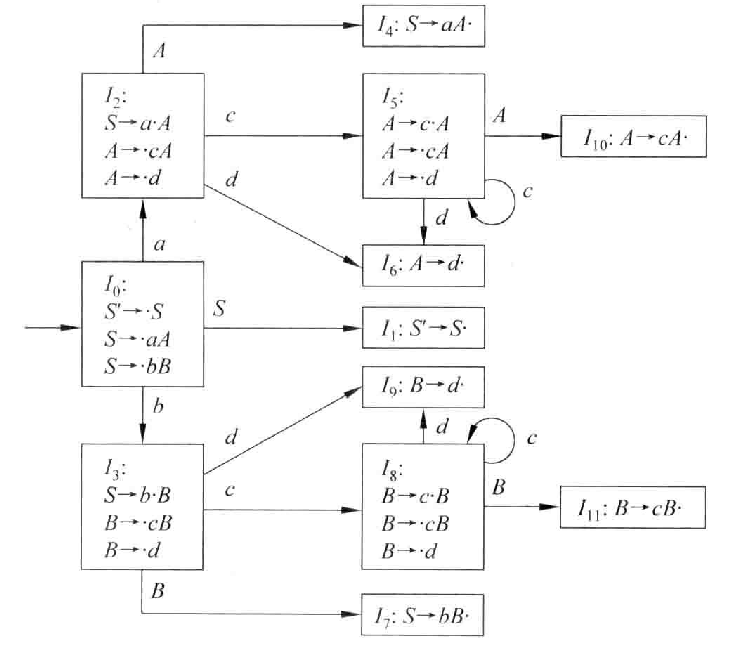
\includegraphics{media/%E8%AF%AD%E6%B3%95%E5%88%86%E6%9E%90/image-20221022152335984.png}

构造的过程是首先以活前缀\$varepsilon\$的有效项目集\$I\emph{0\$为起始,添加\$go(I}0,S),go(I\emph{0,a),go(I}0,b)\$,也就是\$I\emph{1,I}2,I\emph{3\$。然后继续以\$I}1,I\emph{2,I}3\$为起点,得到\$I\emph{4,I}5,I\emph{6,I}7,I\emph{8,I}9\$。然后类似,构建完成整张DFA。

\section*{冲突,SLR(1),LR(0)}

DFA构建完成后,可能存在冲突,例如对于项目集\$I =\{ X rightarrow alpha bullet b beta, quad A rightarrow alpha bullet, quad B rightarrow beta bullet\}\$,存在:

\begin{itemize}
\item 移进-规约冲突:不知道应该移进b还是规约为A或B
\item 规约-规约冲突:不知道应该规约为A还是B
\end{itemize}

如果出现这样的问题,那么不向前看任何符号的LR(0)分析方法是解决不了的。一个缓兵之计是通过FOLLOW集来进行区分,如上面的例子中若A、B的FOLLOW集不存在交集,问题就得到了解决。这种解决办法是通过简单的向前看一个符号来达到的,因此称作SLR(1)分析方法。

如果没有这样的问题,那文法就可以通过LR(0)分析方法解决,也就是,文法的每个有效项目集都满足:要么所有元素都是移进-待约项目,要么只含有唯一的规约项目。

\section*{构建SLR(1)分析表}

\begin{enumerate}
\item 构造 \$G \textasciicircum{}\{prime\}\$ 的 \$L R ( 0 )\$ 项目集规范族 \$C =left\{ I \_0, I \_1, ldots, I \_\{ n \}right\}\$ 。
\item 对于状态\$i\$(对应于项目集\$I\emph{i\$的状态)的分析动作如下:
a) 若 \$A rightarrow alpha cdot a beta in I}i\$,\$a\$为终结符,且 \$g oleft(I\emph{i, aright)=I}j\$, 则置 \$operatorname\{action\}[i, a]=S j\$,表示移入栈一个符号,与此同时将状态\$j\$入栈
b) 若 \$A rightarrow alpha cdot in I \_\{ i \}\$, 则对所有 \$a in F O L L O W ( A )\$, 置 \$operatorname\{action\}[ i , a ]= R(A rightarrow alpha)\$,表示利用生成式\$A rightarrow alpha\$进行规约。
c) 若 \$S \textasciicircum{}\{prime\} rightarrow S in in I \_\{ i \}\$, 则置 \$operatorname\{action\}[ i , S = A C C\$,表示分析成功
\item 若 \$operatorname\{go\}left( I \_\{ i \}, A right)= I \_\{ j \}\$,\$A\$ 为非终结符,则置 \$operatorname\{goto\}[ i , A ]= j\$
\item 分析表中凡不能用规则 \$2 、 3\$ 填入信息的空白表项, 均置出错标志 error。
\item 分析程序的初态是包含项目 \$S \textasciicircum{}\{prime\} rightarrow S\$ 的有效项目集所对应的状态。
\end{enumerate}

构建完成的表若不存在冲突,那么得到的就是一张SLR(1)分析表,文法是SLR(1)文法。

\end{document}
